

\section{Knowledge Graphs}
\label{sec:fundamentals_knowledge_graphs}

\acrfullpl{kg} represent information as structured networks. In these networks, nodes typically denote entities such as individuals, locations, publications, or abstract concepts, while the edges signify the relationships that connect these entities \cite{banerjee_knowledge_2024,pan_unifying_2024}. Although there are numerous definitions for \glspl{kg}, many prominent implementations are modeled using the \gls{rdf} \cite{ehrlinger_towards_2016}. \gls{rdf} provides a graph-based data model standardized by the World Wide Web Consortium (W3C) \cite{wood_rdf_2014}. Consequently, for the scope of this thesis, the term \gls{kg} will specifically refer to an \gls{rdf} graph.

The fundamental unit of an \gls{rdf} graph is the \emph{triple}, a tuple comprising three components: a subject, a predicate, and an object \cite{pan_unifying_2024,wood_rdf_2014,ji_survey_2022}. Following the W3C standard, an \gls{rdf} graph G is formally defined as a set of such triples:
\[
G = \{\, t = (s, p, o) \mid s \in \mathcal{I} \cup \mathcal{B},\; p \in \mathcal{I},\; o \in \mathcal{I} \cup \mathcal{B} \cup \mathcal{L} \,\},
\]
where:
\begin{itemize}
  \item \(\mathcal{I}\) is the set of \glspl{iri}, which uniquely identify resources,
  \item \(\mathcal{B}\) is the set of blank nodes representing resources without a global identifier,
  \item \(\mathcal{L}\) is the set of literals, which are atomic pieces of information (e.g., strings, numbers).
\end{itemize}

Furthermore, a triple \(t = (s, p, o)\) consists of:
\begin{itemize}
  \item \emph{Subject} \(s\): The resource being described, which is either an \gls{iri} or a blank node.
  \item \emph{Predicate} \(p\): A property (or relation) represented as an \gls{iri} that links the subject to the object.
  \item \emph{Object} \(o\): The target or value of the relationship, which may be an \gls{iri}, a blank node, or a literal.
\end{itemize}

The key characteristics of a \gls{kg} have been expressed by \autocite{verma_scholarly_2023}: 
\begin{itemize}
    \item The structure of a \gls{kg} depends on the use of an ontology, which defines the concepts, properties, and associations across a single or multiple domains.
    \item A \gls{kg} is formulated in a triple format and is often stored as an \gls{rdf} graph.
    \item To create the \gls{kg}, knowledge is curated from structured and unstructured sources.
    \item The \gls{kg} is stored in a graph database management system and queried using adaptive querying languages such as CYPHER, SPARQL, SQL, and API calls to retrieve data from the graph.
\end{itemize}

\subsection{Research Knowledge Graphs}

\glspl{kg} are classified based on the information they store. Several categories are recognized in the literature \cite{pan_unifying_2024}: \emph{Encyclopedic \glspl{kg}} aim to represent real-world knowledge, often integrating information from diverse sources like encyclopedias, expert input, and databases. \emph{Commonsense \glspl{kg}} focus on modeling tacit, everyday knowledge and the relationships between common concepts. \emph{Domain-specific \glspl{kg}} contain specialized information pertinent to particular fields. Furthermore, \emph{Multi-modal \glspl{kg}} extend the traditional graph structure to incorporate information from various modalities, including images, audio, and video.

Another type of \glspl{kg} are \acrfullpl{rkg}, which are graphs focused on scholarly communication. Although an \gls{rkg} can also store typical data such as people, documents, datasets, and institutions, it also includes relationships between problems, methods, and results. A distinguishing feature is the representation of statements extracted from scientific articles as semantic resources within the graph. These resources are explicitly linked to their source articles, enabling direct traceability of information provenance. \cite{auer_towards_2018}

\textcite{karras_divide_2023} propose a categorization of \glspl{rkg} into \emph{generic} and \emph{specific} types. Generic \glspl{rkg} primarily utilize bibliographic metadata to structure entities and relationships. Prominent examples include the \emph{Microsoft Academic Knowledge Graph} \cite{ghidini_microsoft_2019,farber_microsoft_2022}, \emph{OpenAlex} \cite{priem_openalex_2022}, \emph{Springer Nature SciGraph} \cite{hammond_data_2017}, \emph{Semantic Scholar Literature Graph} \cite{kinney_semantic_2023}, \emph{OpenAIRE Research Graph} \cite{manghi_data_2012}, \emph{Research Graph} \cite{aryani_research_2017}, and the \emph{Scholarly Link Exchange (Scholix)} framework \cite{burton_scholix_2017}. In contrast, specific \glspl{rkg} focus on storing detailed scientific data in addition to bibliographic metadata. These graphs are employed to describe and link research artifacts and entities, often tailored to particular scientific topics or domains. Notable examples are \emph{CovidGraph} \cite{domingo-fernandez_covid-19_2021}, \emph{SoftwareKG} \cite{harth_investigating_2020}, the \emph{Computer Science Knowledge Graph (CS-KG)} \cite{sattler_cs-kg_2022}, the \emph{Cooperation Databank (CoDa)} \cite{spadaro_cooperation_2022}, and \emph{OpenBiodiv} \cite{penev_openbiodiv_2019}.


\subsection{The Open Research Knowledge Graph (ORKG)}

Beyond the generic and specific classifications, the \acrfull{orkg} presents a distinct approach by aiming to organize topic-specific scientific data semantically across diverse research domains \cite{karras_divide_2023}.

The \gls{orkg} is an \gls{rkg} that stores scientific articles along with their contributions as semantic units. It provides the infrastructure for acquiring, curating, publishing, and processing semantic scientific knowledge with the goal of making scientific findings more accessible to both humans and machines \cite{jaradeh_open_2019-1}. The graph is publicly accessible through a website\footnote{\url{https://orkg.org/} [last accessed on 21.12.2024]} and is maintained by the \gls{orkg} community. New entries can be added by any user, with entry quality being monitored by administrators. At the time of writing this thesis, the graph contains over 33,800 articles across more than 700 different research fields\footnote{\url{https://orkg.org/stats} [last accessed on 21.12.2024]}.

\paragraph{Data Model} Knowledge in the \gls{orkg} is stored closely following the \gls{rdf} format, meaning that at the core, the graph is stored in triples, which are also referred to as \emph{statements}. As detailed in \autoref{tab:orkg_statements}, each component of a statement accommodates specific types of information. Subjects and objects can represent resources, properties, or classes, whereas predicates are restricted to properties. Literals are used for atomic data, such as text, numbers, or dates, and are used exclusively as objects within statements. Furthermore, the \gls{orkg} system automatically assigns a unique identifier (ID) to each resource, property, class, and literal instance. \cite[21-22]{ilangovan_open_2024}

\begin{table}[t]
\centering
\begin{tabular}{|l|l|l|}
\hline
\textbf{Subject} & \textbf{Predicate} & \textbf{Object} \\ \hline
\{ Resource, Property, Class \} & Property & \{ Resource, Property, Class, Literal \} \\ \hline
\end{tabular}
\caption[Permitted ORKG Statement Types]{The permitted types in ORKG statements for the Subject, Predicate, and Object in a triple, based on \cite[21]{ilangovan_open_2024}.}
\label{tab:orkg_statements}
\end{table}

\paragraph{Content Types} Information stored in the \gls{orkg} is organized using distinct content types. A primary content type is the \emph{paper}. When a paper is added, the system automatically populates associated metadata, including its DOI, title, research field, authors, publication date, venue, and URL. Another crucial content type is the \emph{contribution}, which allows users to add structured data describing the research findings presented in the paper, extending beyond simple metadata. These contributions can subsequently be utilized within \emph{comparisons}, another \gls{orkg} content type. Comparisons facilitate the contrasting of research findings across multiple papers and can be semi-automatically generated by the system to identify shared properties among different contributions. \cite[22]{ilangovan_open_2024}

\paragraph{Contribution Templates} To promote standardization in the way contributions are structured, the \gls{orkg} offers \emph{templates}. These templates implement a subset of the Shapes Constraint Language (SHACL) \cite{knublauch_shapes_2017} and define the expected structure for contributions related to specific types of research descriptions. Intended for creation by domain experts, templates specify constraints and requirements, ensuring consistency and quality in the data entered for contributions within particular research areas. \cite[58-60]{ilangovan_open_2024}

\paragraph{Research Fields} The concept of \emph{research fields} serves as a primary organizational mechanism within the \gls{orkg}. Research fields can be associated with various content types (papers, contributions, comparisons, templates, etc.) to enable the grouping and categorization of related content within the graph. \cite[29-30]{ilangovan_open_2024}

\paragraph{Lists} \emph{Lists} provide another organizational tool in the \gls{orkg}. They allow users to group related papers thematically or for specific purposes without necessarily requiring the addition of detailed structured data for each paper within the list. \cite[28-29]{ilangovan_open_2024}

\begin{figure}
    \centering
    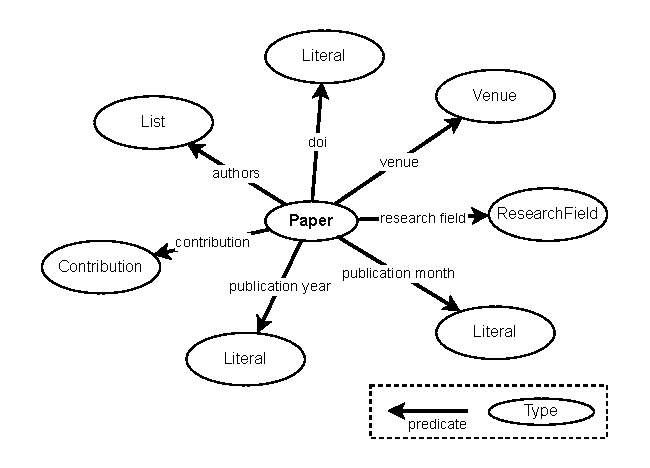
\includegraphics[width=0.7\linewidth]{figures/orkg/figures-orkg_structure.drawio.pdf}
    \caption[Schematic Representation of ORKG Publication Data]{Schematic representation of how publication data is structured in the ORKG, illustrating the root entity \emph{Paper} and its linkage to metadata and \emph{Contribution} entities.}
    \label{fig:orkg_structure}
\end{figure}

\paragraph{Storing Publications} As previously mentioned, scientific publications are represented in the \gls{orkg} using the \emph{paper} content type. Interaction with these paper entities forms the principal mode of engagement with the \gls{orkg} relevant to this thesis. \autoref{fig:orkg_structure} depicts the organizational structure for storing publication data. The diagram illustrates that the paper entity serves as the central node for publication information. All associated data, including metadata and one or more contributions detailing the research content, are linked to this paper entity using statements.

\subsection{The KARAGEN Approach for Question Answering on the ORKG}

\gls{karagen} is an approach for implementing a \gls{qa} system on the \gls{orkg} graph. The goal is to take advantage of the complementary strengths of \glspl{llm} and \gls{kg}. In this relationship, the \gls{kg} provides a structured data foundation in which information is stored in an interconnected network of entities and their relationships. The benefit of the graph is the ability to semantically link information, thus preserving the context and relationships between pieces of knowledge. On the other hand, \glspl{llm} excel in interpreting and generating natural language, with their advantage being that users can formulate their queries in natural language instead of relying on keyword-based queries. \cite{kaplan_combining_2024}

\begin{figure}[t]
    \centering
    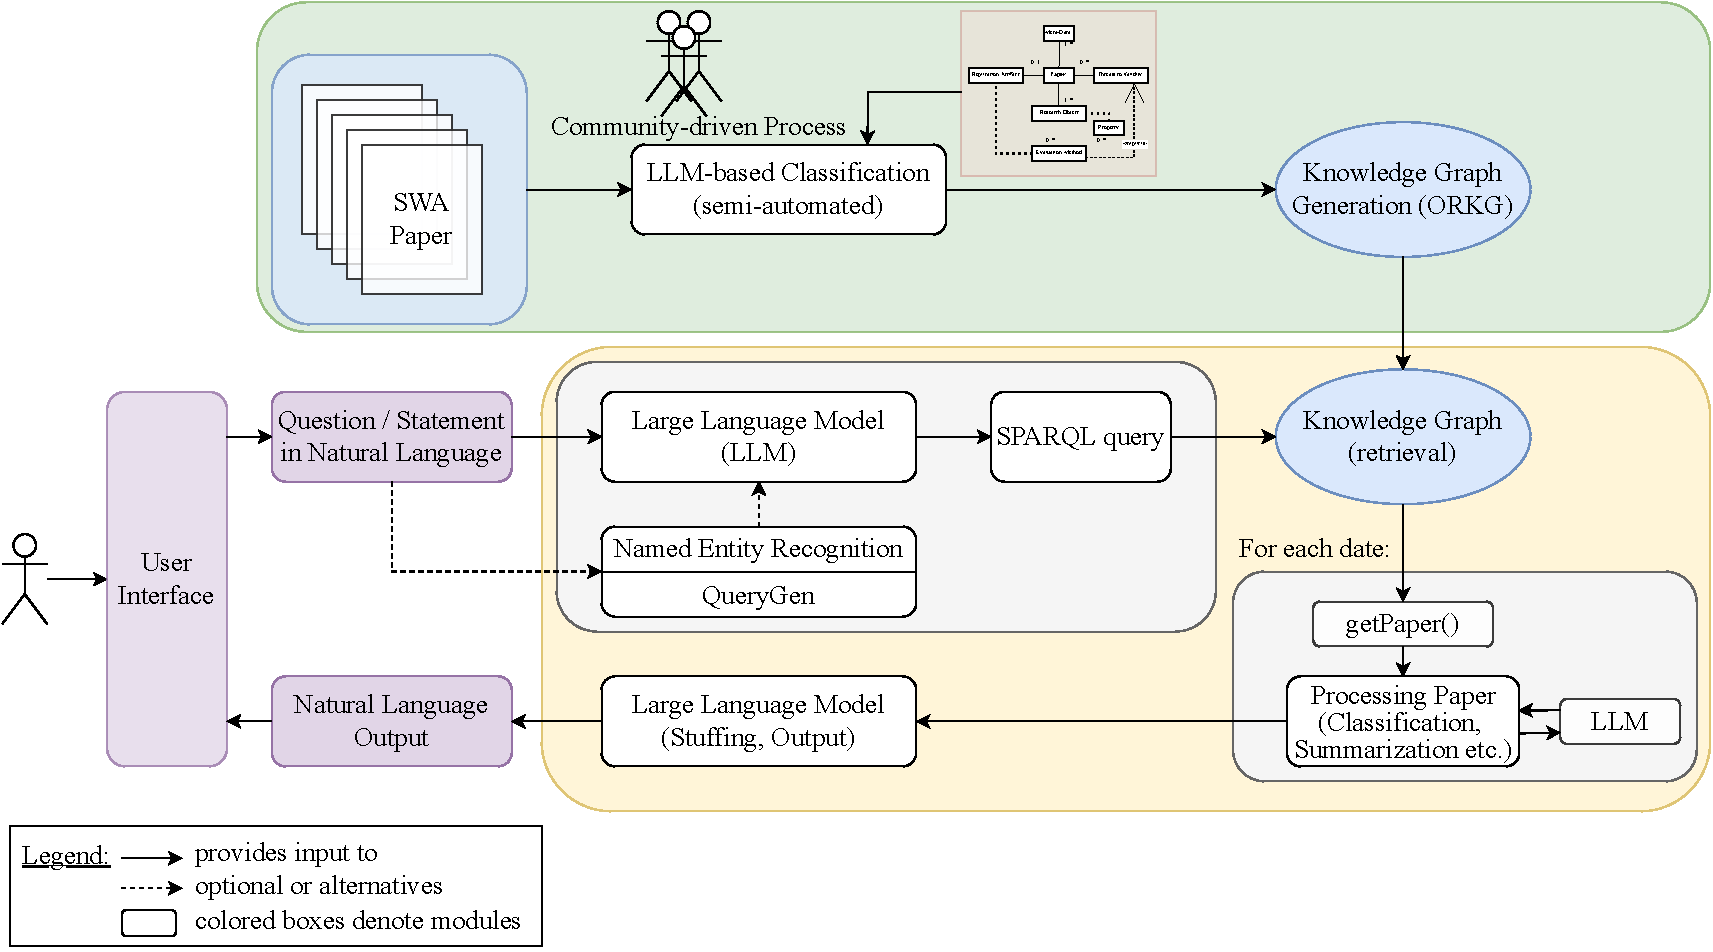
\includegraphics[width=0.95\textwidth]{figures/karagen.pdf}
    \caption[The KARAGEN Approach]{The KARAGEN approach, as proposed by \textcite{kaplan_combining_2024}, consists of two parts for a \gls{llm}-based retrieval on the \gls{orkg}. The green box shows the generation and population of the \gls{orkg}, while the yellow box depicts the \gls{llm}-based retrieval.}
    \label{fig:karagen}
\end{figure}

The \gls{karagen} approach is illustrated in \autoref{fig:karagen} and is composed of two parts: 1) Knowledge Graph Generation and Population and 2) Knowledge Retrieval. The following explanations are based on the descriptions provided by \textcite{kaplan_combining_2024}.

\paragraph{Knowledge Graph Generation and Population} This component is responsible for populating the \gls{orkg} with information through a semi-automated process, where users are supported by \gls{llm}-based classification. In the case of the \gls{orkg}, adding information about research papers is facilitated through templates. This means that either users or machines can fill in the required information into these templates, which are then stored in the graph as a contribution to the research paper.

\paragraph{Knowledge Retrieval} This component handles the retrieval and processing of knowledge from the graph. Users can submit queries in natural language, which are then processed using an \gls{llm}. The retrieval process may involve several steps, such as generating graph queries by matching natural language elements to graph components. Optionally, a knowledge enhancement component can be incorporated to transform and generate information. Finally, the system generates a response for the user. During this retrieval process, sources can be added to indicate the origin of the data and ensure traceability.

% In the following, we present the core concepts of the \gls{orkg}. This information is derived from \cite{ilangovan_open_2024} and the official \gls{orkg} website\footnote{\url{https://orkg.org/about} [last accessed on 21.12.2024]}.

% A recent study by \textcite{verma_scholarly_2023} reviewed 10 \glspl{rkg} that support scholarly infrastructures and found that nearly all used RDF for data representation. The study also highlighted that the core research-related entities across these graphs are quite similar, generally grouping into eight categories. The first group, \emph{People}, involves individuals such as authors and researchers. The second group, \emph{Publications}, relates to scholarly outputs like journal articles and conference papers. The third group, \emph{Organizations}, includes universities, research institutes, and other bodies that researchers belong to. The fourth group, \emph{Events}, covers academic gatherings like conferences and workshops. The fifth group, \emph{Datasets}, refers to digital collections or platforms where publications, data, and related resources are stored. The sixth group, \emph{Publishers \& Venues}, encompasses journals, conference venues, and other forms of publishers.

% TODO Add typical structure of a RKG \cite{verma_scholarly_2023}



% A \gls{kg} is an extended form of an ontology providing richer entity descriptions at the instance level \cite{ilangovan_open_2024}. 

% Mathematically speaking, a \gls{kg} stores structured knowledge as a collection of triples \(KG = \{(h,r,t) \subseteq \varepsilon \times R \times \varepsilon \} \), where \(\varepsilon\) denotes the entities and \(R\) the relation between the entities \cite{pan_unifying_2024}. These entities and their relationships are organized in a directed graph (\(G\)), defined as \(G = (V, E)\). In this graph, the vertices (\(V\)) correspond to the entities, and the edges (\(E\)) denote the relationships between them. Intuitively, a fact in the knowledge graph is formed by two entities connected by a relationship \cite{abu-salih_domain-specific_2021}.

% \Glspl{kg} have become an emerging technology in industry and in academia as they enable data to be organized \enquote{in a flexible, fine-grained, context-sensitive, and semantic representation to be understandable, processable, and usable by humans and machines \cite{karras_divide_2023}}.

% - A scholarly \gls{kg} is a type of graph that contains bibliographic information \cite{banerjee_dblp-quad_2023}. Some well known scholarly \glspl{kg} are the Microsoft Academic Graph, OpenAlex, ORKG, and DBLP.

% - The DBLP \gls{kg} includes bibliographic information on a wide range of topics within the field of computer science. It mainly consists of two entities \emph{Person} and \emph{Publication} \cite{banerjee_dblp-quad_2023}.  
% According to \textcite{taye_understanding_2010}, the semantic web aims to extend the current web by representing the information in both a human and machine-readable format. The backbone of the semantic web is formed by \emph{ontologies} by offering a shared conceptualization of a domain. An ontology consists of the following components:

% \begin{enumerate}
%     \item \emph{Concepts} are also referred to as classes or terms and represent abstract groups, sets, or collections of objects within a domain. They are organized hierarchically with parent and child relationships.
%     \item \emph{Instances} or individuals represent specific objects or elements of a concept.
%     \item \emph{Relations} or slots define how concepts are related to one another.
%     \item \emph{Axioms} are used to impose constraints on the values of concepts or instances. These are usually expressed in logic-based languages and ensure consistency within the ontology.
% \end{enumerate}

% \gls{rdf} is described as the first layer of the Semantic Web architecture \cite{taye_understanding_2010}. It provides the framework for representing metadata and semantics in a machine-readable format and can be applied to semi-formally describe ontologies. At the core of \gls{rdf} are triples, which are statements in the form of \((subject, predicate, object)\) \cite{wood_rdf_2014}. A \emph{subject} is the resource that is being defined, which can be either an \gls{iri} or a blank node. A \emph{predicate} is the property or relation between the subject and the object in the form of an \gls{iri}. The \emph{object} is the value or target of the relationship and can be either an \gls{iri}, a blank node, or a literal. A \gls{iri} acts as a unique identifier for resources, while literals are atomic pieces of information. Blank nodes are used to represent resources that do not have a unique identifier. 

% Combined as a set, triples form a \gls{rdf} graph which is a directed graph where the nodes represent entities and the edges represent the relationships between them \cite{hogan_knowledge_2022, paulheim_knowledge_2016, barrasa_building_2023}. When such a graph accumulates data to convey knowledge about the real world, making it comprehensible to both humans and machines, it is referred to as a \gls{kg}. 